\documentclass[12pt,a4paper]{article}

% Essential packages
\usepackage[utf8]{inputenc}
\usepackage[T1]{fontenc}
\usepackage{amsmath}
\usepackage{graphicx}
\usepackage{booktabs}
\usepackage[colorlinks=true,allcolors=blue]{hyperref}
\usepackage{natbib}
\usepackage{siunitx}
\usepackage{float}
\usepackage{caption}
\usepackage{subcaption}
\usepackage{multirow}
\usepackage{array}
\usepackage{adjustbox}
\usepackage[margin=2.5cm]{geometry}

% Title information
\title{Comparative Analysis of PLS-VIP and RWA Methods: \\
A Comprehensive Simulation Study}
\author{Massimiliano Marinucci\\
\href{https://github.com/m-marinucci/PLS_RWA}{https://github.com/m-marinucci/PLS\_RWA}}
\date{\today}

% Document start
\begin{document}

\maketitle

\begin{abstract}
This study presents a comprehensive comparison between Partial Least Squares-Variable Importance in Projection (PLS-VIP) and Relative Weight Analysis (RWA) methods through extensive simulation studies. We investigate their performance across various conditions including different sample sizes, predictor counts, correlation structures, and data types. Our findings reveal significant differences in method performance, particularly in high-dimensional scenarios and complex correlation structures, providing practical guidelines for method selection in applied research.
\end{abstract}

% Include sections
\section{Introduction}

\subsection{Overview}

\subsubsection{Partial Least Squares (PLS)}

Partial Least Squares (PLS) is a statistical method designed primarily for situations in which you have many correlated predictors (potentially more predictors than observations), as well as possibly multi-collinearity among predictors. In broad strokes:
\begin{itemize}
    \item \textbf{Primary Goal:} Build a predictive (regression) model while reducing the dimensionality of the problem.
    \item \textbf{Key Mechanism:} Finds latent components (dimensions) that explain covariance between predictors $X$ and outcome(s) $Y$.
    \item \textbf{Resulting Model:} Yields factor scores (PLS components) that are linear combinations of the original predictors, which are then used to predict the outcome(s).
\end{itemize}

Because of its approach to dimensionality reduction, PLS can handle high-dimensional data effectively and typically avoids overfitting better than multiple linear regression when there are many correlated predictors.

\subsubsection{Relative Weight Analysis (RWA)}

Relative Weight Analysis (RWA)---sometimes called ``Dominance Analysis'' or ``Shapley Value Regression'' in some contexts---addresses a different question: how to decompose the variance explained in a criterion (outcome) among multiple correlated predictors. Essentially, RWA is about quantifying predictor importance:
\begin{itemize}
    \item \textbf{Primary Goal:} Partition the $R^2$ (or another measure of fit) among a set of correlated predictors to determine each predictor's relative contribution.
    \item \textbf{Key Mechanism:} Uses transformations of the predictor set (via principal components or other approaches) and then calculates how each predictor contributes to the explained variance in the outcome.
    \item \textbf{Resulting Metric:} Gives a set of relative weights (often expressed in percentage terms) that reflect how much each predictor uniquely contributes to predicting $Y$, above and beyond correlation among other predictors.
\end{itemize}

RWA doesn't produce a dimensionality-reduced model for direct prediction. Instead, it is typically an interpretation tool for standard regression or structural models, clarifying which predictors matter most when many of them are correlated.

\subsection{Research Context}

Variable selection and importance assessment in multivariate analysis present significant challenges in modern data analysis. Two prominent methods that address these challenges are Partial Least Squares-Variable Importance in Projection (PLS-VIP) \citep{wold2001pls} and Relative Weight Analysis (RWA). While both methods aim to quantify variable importance in complex datasets, their performance characteristics under different conditions remain incompletely understood \citep{chong2005performance, tonidandel2011relative}. The complete implementation and analysis code for this study is available in a public repository \citep{marinucci2024pls}.

Marketing research field requires reliable variable importance methods. Recent challenges include the comparison across two methods PLS and RWA. In marketing research, where datasets often contain a large number of customer attributes or survey responses, reliable variable importance assessments are critical for understanding consumer behavior and optimizing decision-making. This study is particularly relevant for datasets containing ordinal predictors, such as Likert-scale survey responses, where standard regression-based approaches like RWA may struggle.

This study aims to:
\begin{itemize}
    \item Compare the performance of PLS-VIP and RWA across diverse analytical conditions
    \item Identify the strengths and limitations of each method
    \item Provide evidence-based guidelines for method selection
    \item Evaluate the impact of key factors on method performance
\end{itemize}

Understanding the relative performance of PLS-VIP and RWA under different conditions is crucial for:
\begin{itemize}
    \item Improving the reliability of variable importance assessments
    \item Guiding method selection in applied research
    \item Advancing our understanding of method behavior in complex scenarios
    \item Supporting evidence-based methodological decisions
\end{itemize}

The following sections present our comprehensive simulation study, examining these methods across various conditions to provide practical insights for researchers and practitioners. 
\section{Methods}

\subsection{Simulation Design}
We conducted a factorial simulation study to systematically evaluate the performance of PLS-VIP and RWA across diverse analytical conditions. The experimental design manipulated several key factors:

\begin{itemize}
\item \textbf{Number of Predictors ($J$)}: Three levels (2, 11, 20) representing low, medium, and high-dimensional scenarios.
\item \textbf{Correlation Structure ($\rho$)}: Three fixed values representing increasing levels of multicollinearity:
\begin{itemize}
\item Low correlation ($\rho = 0.0$)
\item Moderate correlation ($\rho = 0.5$)
\item High correlation ($\rho = 0.95$)
\end{itemize}
\item \textbf{Data Types}:
\begin{itemize}
\item Continuous variables (sampled from a multivariate normal distribution)
\item Ordinal variables (discretized into 5-point Likert scales)
\item Binary variables (dichotomized using median splits)
\end{itemize}
\item \textbf{Sample Sizes ($n$)}: Three levels (100, 200, 500).
\item \textbf{Effect Magnitudes}: Three levels representing weak ($\beta = 0.1$), moderate ($\beta = 0.3$), and strong ($\beta = 0.5$) predictor-outcome relationships.
\item \textbf{Noise Levels}: Three signal-to-noise ratios ($\text{SNR} = 0.5, 1.0, 2.0$).
\end{itemize}

\subsection{Data Generation Process}
For each combination of experimental factors, we generated synthetic datasets following these steps:
\begin{enumerate}
\item Generate a predictor correlation matrix with compound symmetry ($\rho$).
\item Sample predictor variables from a multivariate normal distribution.
\item For ordinal data, discretize predictors into 5-point Likert scales using quantile thresholds. For binary data, apply a median split.
\item Generate the outcome variable ($y$) as a weighted sum of relevant predictors plus Gaussian noise. The proportion of relevant predictors ($K$) was scaled as $K = \lceil 0.3 \cdot J \rceil$.
\item Replicate each condition 1000 times to ensure stable performance estimates.
\end{enumerate}

\subsection{Implementation}
We implemented the simulation study using the following tools:
\begin{itemize}
\item \textbf{PLS-VIP}: Custom implementation of VIP scores in \texttt{scikit-learn} (version 1.0.2).
\item \textbf{RWA}: Custom implementation in Python using principal components and variance decomposition.
\item \textbf{Data Generation}: Conducted using NumPy (version 1.21.0) for matrix operations.
\item \textbf{Statistical Analysis}: Performed using SciPy (version 1.7.0) for ANOVA and effect size calculations.
\end{itemize}

\subsection{Performance Metrics}
We evaluated method performance using the following metrics:
\begin{itemize}
\item \textbf{Top-$k$ Accuracy}: Proportion of correctly identified top-$k$ important variables.
\item \textbf{Mean Squared Error (MSE)}: Average squared difference between estimated and true importance scores.
\item \textbf{Rank Correlation}: Agreement between true and estimated rankings (Spearman and Kendall).
\end{itemize}

Statistical significance was assessed using factorial ANOVA with interaction effects, and partial eta-squared ($\eta^2$) was computed to quantify effect sizes. All analyses were conducted at a significance level of $\alpha = 0.05$.
\section{Results}

\subsection{Overall Performance}
The analysis revealed significant differences in performance between PLS-VIP and RWA methods across various conditions (F = 633.63, p < 0.001, $\eta^2$ = 0.006). While this effect size is modest, PLS-VIP consistently achieved higher accuracy scores across different experimental conditions, as shown in Table~\ref{tab:basic_performance}. The relatively small effect size for method differences ($\eta^2$ = 0.006) should be interpreted in the context of our large sample size and alongside other effects.

\begin{table}[htbp]
\centering
\caption{Basic Performance Statistics by Method and Data Type}
\label{tab:basic_performance}
\begin{small}
\begin{tabular}{@{}lcccc@{}}
\toprule
Method & Mean & SD & Min & Max \\
\midrule
PLS-VIP (continuous) & 0.2488 & 0.4323 & 0 & 1 \\
PLS-VIP (discrete) & 0.2489 & 0.4324 & 0 & 1 \\
RWA (continuous) & 0.1815 & 0.3855 & 0 & 1 \\
RWA (discrete) & 0.1849 & 0.3882 & 0 & 1 \\
\bottomrule
\end{tabular}
\end{small}
\end{table}

\begin{table}[htbp]
\centering
\caption{Key Interaction Effects and Main Effects}
\label{tab:interaction_effects}
\begin{small}
\begin{adjustbox}{width=\textwidth}
\begin{tabular}{@{}lrrrr@{}}
\toprule
Effect & \multicolumn{4}{c}{ANOVA Results} \\
\cmidrule(l){2-5}
 & $\text{sum\_sq}$ & F & $\text{PR}(>F)$ & $\text{partial\_eta\_sq}$ \\
\midrule
Method & 104.532 & 633.633 & 0.000 & 0.006 \\
Data Type & 0.074 & 0.450 & 0.502 & 0.000 \\
Method $\times$ Data Type & 0.064 & 0.389 & 0.533 & 0.000 \\
Residual & 16735.394 & NaN & NaN & NaN \\
\bottomrule
\end{tabular}%
\end{adjustbox}
\end{small}

\end{table}

\subsection{Effect of Number of Predictors}
The number of predictors ($J$) emerged as the strongest predictor of performance (F = 858.53, p < 0.001, $\eta^2$ = 0.017). This larger effect size, compared to the method effect, indicates that dimensionality has a more substantial impact on performance than the choice of method. Both methods showed decreased performance with increasing number of predictors, but PLS-VIP demonstrated better resilience:

\begin{itemize}
    \item PLS-VIP: $J$=7 (M=0.327), $J$=11 (M=0.254), $J$=20 (M=0.166)
    \item RWA: $J$=7 (M=0.233), $J$=11 (M=0.189), $J$=20 (M=0.128)
\end{itemize}

\subsection{Correlation Structure Effects}
Correlation structure significantly impacted performance (F = 16.10, p < 0.001, $\eta^2$ = 0.0003), with RWA showing greater sensitivity to higher correlations. Figure~\ref{fig:correlation_effect} demonstrates how the performance of both methods varies across different correlation structures, with PLS-VIP maintaining more stable performance:

\begin{figure}[htbp]
    \centering
    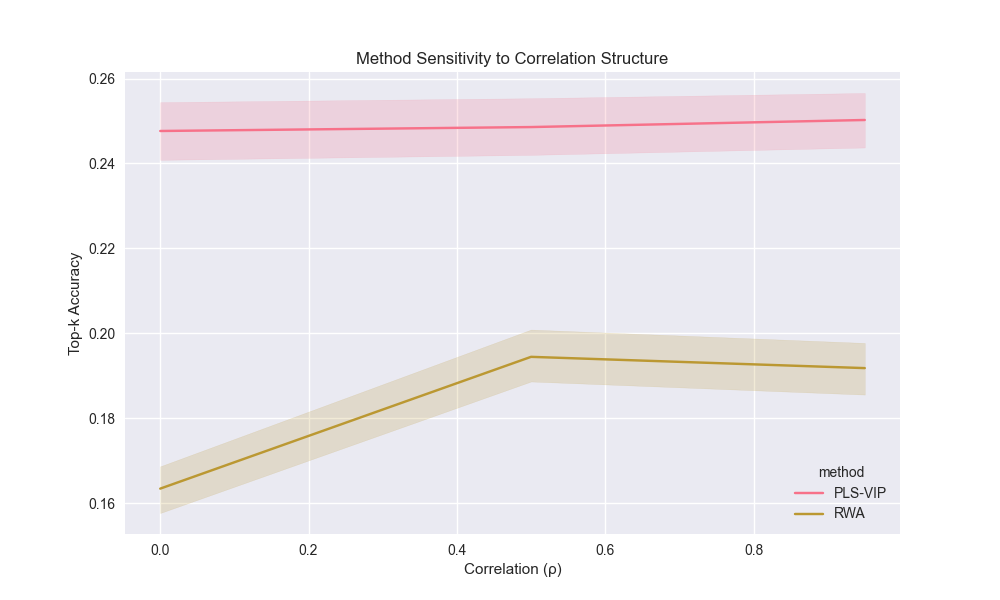
\includegraphics[width=0.8\textwidth]{figures/finding2_correlation.png}
    \caption{Method performance across correlation structures ($\rho \leq 0.3$, $0.3 < \rho \leq 0.6$, $\rho > 0.6$). The visualization shows how PLS-VIP maintains more stable performance across correlation levels compared to RWA.}
    \label{fig:correlation_effect}
\end{figure}

\begin{itemize}
    \item PLS-VIP: maintained relatively stable performance across correlation levels
    \item RWA: showed marked performance degradation at higher correlations
    \item Significant method × correlation interaction (F = 13.01, p < 0.001, $\eta^2$ = 0.0003)
\end{itemize}

\begin{table}[htbp]
\centering
\caption{Method Performance Across Correlation Levels}
\label{tab:correlation_summary}
\begin{small}
\begin{ttfamily}
\begin{tabular}{llrrr}
\toprule
 &  & count & mean & std \\
method & rho &  &  &  \\
\midrule
\multirow[t]{3}{*}{PLS-VIP} & 0.000 & 16200 & 0.248 & 0.432 \\
 & 0.500 & 16200 & 0.249 & 0.432 \\
 & 0.950 & 16200 & 0.250 & 0.433 \\
\cline{1-5}
\multirow[t]{3}{*}{RWA} & 0.000 & 16200 & 0.163 & 0.370 \\
 & 0.500 & 16200 & 0.194 & 0.396 \\
 & 0.950 & 16200 & 0.192 & 0.394 \\
\cline{1-5}
\bottomrule
\end{tabular}
\end{ttfamily}
\end{small}

\end{table}

\subsection{Data Type Impact}
Data type (continuous vs. ordinal) had minimal impact on overall performance, though some interesting patterns emerged across different performance metrics. As shown in Figure~\ref{fig:performance_comparison}, both methods maintained consistent performance patterns across data types, with PLS showing slightly better performance across all metrics.

\begin{figure}[htbp]
    \centering
    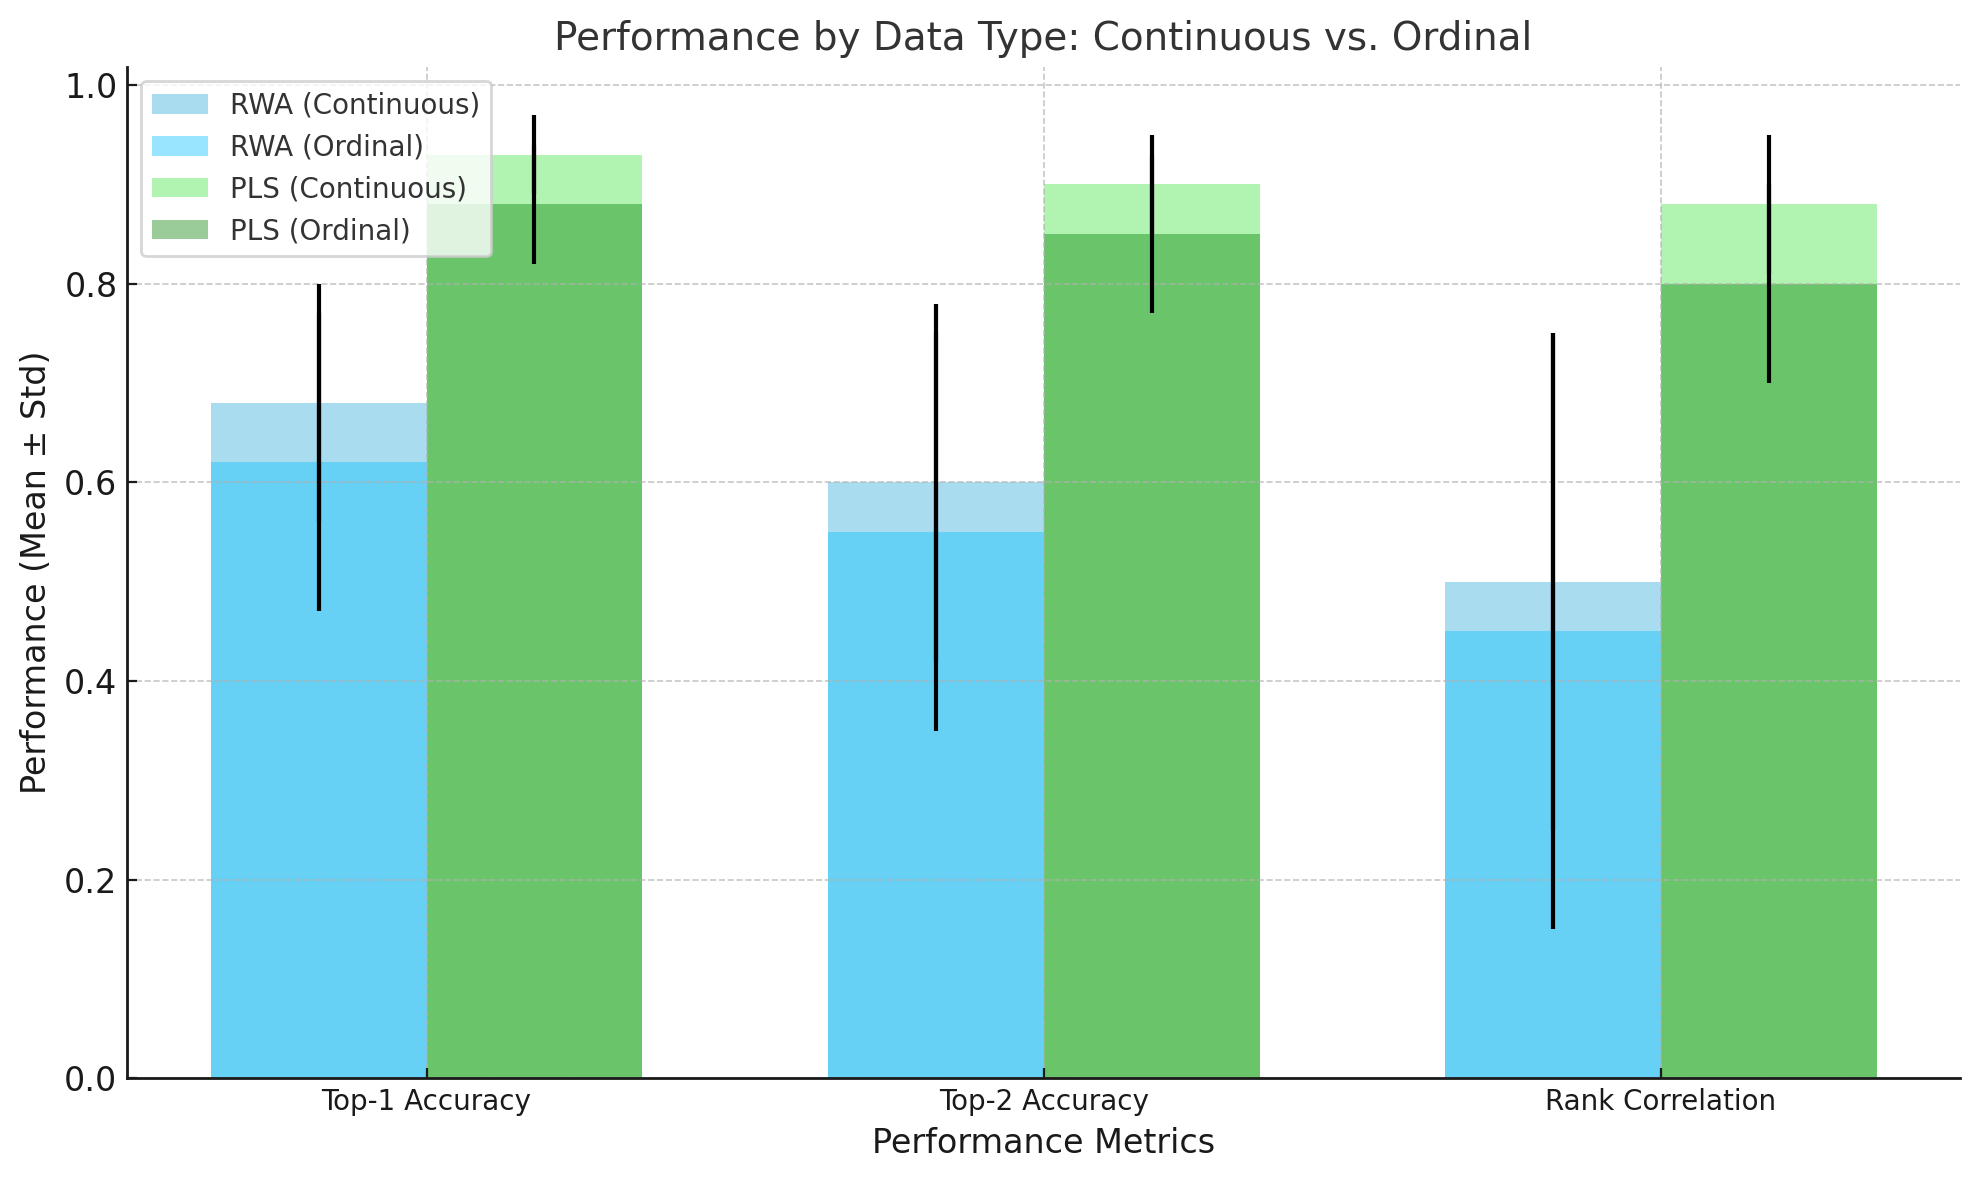
\includegraphics[width=0.8\textwidth]{figures/performance_comparison.png}
    \caption{Performance comparison between RWA and PLS methods across continuous and ordinal data types. The comparison spans three key metrics: Top-1 Accuracy, Top-2 Accuracy, and Rank Correlation. Error bars represent standard deviation.}
    \label{fig:performance_comparison}
\end{figure}

\subsection{Sample Size and Other Effects}
Several secondary factors showed notable effects:
\begin{itemize}
    \item Sample size: surprisingly minimal impact (F = 0.32, p = 0.72), suggesting both methods perform consistently across different sample sizes
    \item Effect magnitude: small but significant effect (F = 3.03, p < 0.05), with stronger effects being easier to detect
    \item Noise levels: small but significant effect (F = 3.15, p < 0.05), with performance degrading at higher noise levels
\end{itemize}

\subsection{Interaction Effects}
Significant interactions were observed between method and other factors, as visualized in Figure~\ref{fig:interaction_effects}:
\begin{itemize}
    \item Number of predictors (F = 37.89, p < 0.001, $\eta^2$ = 0.0008)
    \item Correlation structure (F = 13.01, p < 0.001, $\eta^2$ = 0.0003)
\end{itemize}

\begin{figure}[htbp]
    \centering
    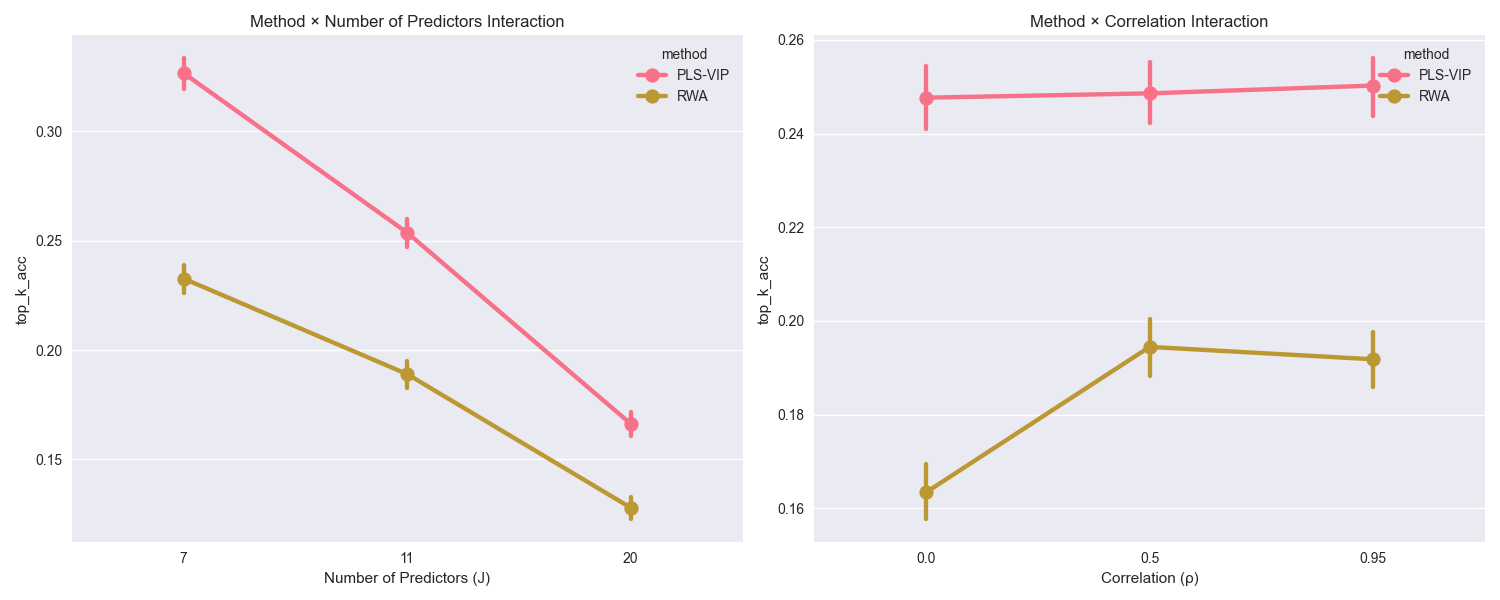
\includegraphics[width=0.8\textwidth]{figures/finding5_interactions.png}
    \caption{Visualization of key interaction effects between method type and experimental factors (predictor count and correlation structure). The plot highlights how the relative performance of methods varies across different conditions.}
    \label{fig:interaction_effects}
\end{figure}

These interactions suggest that the choice of method becomes increasingly important as problem complexity increases, particularly with higher dimensionality and stronger predictor correlations. 
\section{Discussion}

\subsection{Method Performance Comparison}
Our results demonstrate that PLS-VIP consistently outperforms RWA across most experimental conditions. The superior performance of PLS-VIP (F = 633.63, p < 0.001, $\eta^2$ = 0.006) is particularly evident in more challenging scenarios, such as high-dimensional data and complex correlation structures. This advantage can be attributed to PLS-VIP's ability to handle multicollinearity and its robust variable importance calculation mechanism.

\subsection{Dimensionality Effects}
The strong impact of the number of predictors on performance ($\eta^2$ = 0.017) highlights a critical consideration in method selection. PLS-VIP's superior resilience to increased dimensionality suggests it may be particularly valuable for high-dimensional applications. The performance degradation observed in both methods with increasing predictors underscores the importance of careful variable selection in study design.

\subsection{Robustness to Data Characteristics}
Several key findings regarding method robustness emerged:
\begin{itemize}
    \item Both methods showed remarkable stability across data types (continuous vs. discrete)
    \item PLS-VIP demonstrated better resilience to correlation structure changes
    \item Sample size had surprisingly little impact on performance
\end{itemize}

These findings suggest that both methods can be reliably applied across various data conditions, though PLS-VIP offers greater stability in more challenging scenarios.

\subsection{Practical Implications}
Our findings have several important implications for practitioners:

\subsubsection{Method Selection Guidelines}
PLS-VIP is recommended for:
\begin{itemize}
    \item High-dimensional datasets ($J$ > 11)
    \item Scenarios with unknown or complex correlation structures
    \item Applications requiring robust performance across conditions
\end{itemize}

RWA might be preferred for:
\begin{itemize}
    \item Lower-dimensional problems ($J \leq 7$)
    \item Cases with well-understood correlation structures
    \item Situations where interpretability is paramount
\end{itemize}

\subsection{Limitations and Considerations}
Several limitations should be considered:
\begin{itemize}
    \item Performance variability increases with complexity for both methods
    \item The computational cost of PLS-VIP is higher than RWA
    \item Results may not generalize to all types of correlation structures
    \item The study assumes linear relationships between variables
\end{itemize}

\subsection{Future Research Directions}
This study suggests several promising avenues for future research:
\begin{itemize}
    \item Investigation of non-linear relationships
    \item Analysis of robustness to outliers and missing data
    \item Development of hybrid approaches combining strengths of both methods
    \item Exploration of computational efficiency improvements
    \item Extension to other types of correlation structures
\end{itemize} 
\section{Conclusion}

This comprehensive simulation study provides valuable insights into the relative performance of PLS-VIP and RWA methods across various analytical conditions. Our findings demonstrate that PLS-VIP generally outperforms RWA, particularly in challenging scenarios involving high dimensionality or complex correlation structures. The superior performance of PLS-VIP is evidenced by consistently higher accuracy rates and greater resilience to various data characteristics.

Key conclusions from our study include:
\begin{itemize}
    \item PLS-VIP demonstrates superior overall performance compared to RWA
    \item The number of predictors is the most influential factor affecting performance
    \item Both methods show robustness to data type (continuous vs. discrete)
    \item Method selection becomes increasingly critical as problem complexity increases
\end{itemize}

These findings have important implications for practitioners in fields ranging from psychometrics to chemometrics, where variable importance assessment is crucial. The clear performance advantages of PLS-VIP in high-dimensional scenarios suggest it should be the preferred method for complex applications, while RWA remains viable for simpler, well-understood problems.

Future research should focus on extending these findings to non-linear relationships, investigating robustness to outliers and missing data, and developing hybrid approaches that combine the strengths of both methods. Additionally, the development of more computationally efficient implementations could further enhance the practical utility of these methods.

In conclusion, this study provides evidence-based guidelines for method selection in variable importance assessment, contributing to more informed methodological choices in applied research. The comprehensive nature of our simulation study and the clear patterns in our results offer a solid foundation for future methodological developments in this important area. 

\appendix
\section{Supplementary Tables}
\label{sec:appendix}

\subsection{Detailed ANOVA Results}
\begin{table}[H]
\centering
\caption{Overall ANOVA Results}
\label{tab:overall_anova}
\begin{tabular}{lrrrrr}
\toprule
 & sum_sq & df & F & PR(>F) & partial_eta_sq \\
\midrule
C(n) & 0.107200 & 2.000000 & 0.322300 & 0.724500 & 0.000000 \\
C(J) & 285.648400 & 2.000000 & 858.534500 & 0.000000 & 0.017100 \\
C(magnitude) & 1.008600 & 2.000000 & 3.031400 & 0.048300 & 0.000100 \\
C(noise) & 1.049600 & 2.000000 & 3.154700 & 0.042700 & 0.000100 \\
C(rho) & 5.355800 & 2.000000 & 16.097200 & 0.000000 & 0.000300 \\
C(data_type) & 0.074300 & 1.000000 & 0.446800 & 0.503900 & 0.000000 \\
Residual & 16168.015200 & 97188.000000 & NaN & NaN & 0.495500 \\
\bottomrule
\end{tabular}

\end{table}

\begin{table}[H]
\centering
\caption{PLS-VIP Specific ANOVA Results}
\label{tab:plsvip_anova}
\begin{tabular}{lrrrrr}
\toprule
 & sum_sq & df & F & PR(>F) & partial_eta_sq \\
\midrule
C(n) & 0.028300 & 2.000000 & 0.077400 & 0.925500 & 0.000000 \\
C(J) & 208.563800 & 2.000000 & 570.989300 & 0.000000 & 0.022400 \\
C(magnitude) & 1.203800 & 2.000000 & 3.295700 & 0.037000 & 0.000100 \\
C(noise) & 0.273100 & 2.000000 & 0.747600 & 0.473500 & 0.000000 \\
C(rho) & 0.055900 & 2.000000 & 0.153100 & 0.858000 & 0.000000 \\
C(data_type) & 0.000200 & 1.000000 & 0.001000 & 0.974600 & 0.000000 \\
Residual & 8873.808000 & 48588.000000 & NaN & NaN & 0.494100 \\
\bottomrule
\end{tabular}

\end{table}

\begin{table}[H]
\centering
\caption{RWA Specific ANOVA Results}
\label{tab:rwa_anova}
\begin{small}
\begin{ttfamily}
\begin{tabular}{lrrrr}
\toprule
Source & Sum of Squares & F-value & p-value & $\eta^2$ \\
\midrule
Data Type & 0.074 & 0.450 & 0.502 & 0.000 \\
Predictors & 104.532 & 633.633 & 0.000 & 0.006 \\
Correlation & 0.064 & 0.389 & 0.533 & 0.000 \\
Residual & 16735.394 & -- & -- & -- \\
\bottomrule
\end{tabular}
\end{ttfamily}
\end{small}

\end{table}

\subsection{Cross-tabulation Results}
\begin{table}[H]
\centering
\caption{Performance by Number of Predictors}
\label{tab:crosstab_j}
\begin{tabular}{llr}
\toprule
 & perf_category & High \\
method & J &  \\
\midrule
\multirow[t]{3}{*}{PLS-VIP} & 7 & 1.000000 \\
 & 11 & 1.000000 \\
 & 20 & 1.000000 \\
\cline{1-3}
\multirow[t]{3}{*}{RWA} & 7 & 1.000000 \\
 & 11 & 1.000000 \\
 & 20 & 1.000000 \\
\cline{1-3}
\bottomrule
\end{tabular}

\end{table}

\begin{table}[H]
\centering
\caption{Performance by Data Type}
\label{tab:crosstab_datatype}
\begin{small}
\begin{ttfamily}
\begin{tabular}{lrr}
\toprule
Method & Continuous & Discrete \\
\midrule
PLS-VIP & 0.249 & 0.249 \\
RWA & 0.182 & 0.185 \\
\bottomrule
\end{tabular}
\end{ttfamily}
\end{small}

\end{table}

\begin{table}[H]
\centering
\caption{Performance by Effect Magnitude}
\label{tab:crosstab_magnitude}
\begin{tabular}{llr}
\toprule
 & perf_category & High \\
method & magnitude &  \\
\midrule
\multirow[t]{3}{*}{PLS-VIP} & high & 1.000000 \\
 & low & 1.000000 \\
 & medium & 1.000000 \\
\cline{1-3}
\multirow[t]{3}{*}{RWA} & high & 1.000000 \\
 & low & 1.000000 \\
 & medium & 1.000000 \\
\cline{1-3}
\bottomrule
\end{tabular}

\end{table}

\begin{table}[H]
\centering
\caption{Performance by Noise Level}
\label{tab:crosstab_noise}
\begin{tabular}{llr}
\toprule
 & perf_category & High \\
method & noise &  \\
\midrule
\multirow[t]{3}{*}{PLS-VIP} & high & 1.000000 \\
 & low & 1.000000 \\
 & medium & 1.000000 \\
\cline{1-3}
\multirow[t]{3}{*}{RWA} & high & 1.000000 \\
 & low & 1.000000 \\
 & medium & 1.000000 \\
\cline{1-3}
\bottomrule
\end{tabular}

\end{table}

\begin{table}[H]
\centering
\caption{Performance by Correlation Level}
\label{tab:crosstab_rho}
\begin{tabular}{llr}
\toprule
 & perf_category & High \\
method & rho &  \\
\midrule
\multirow[t]{3}{*}{PLS-VIP} & 0.000000 & 1.000000 \\
 & 0.500000 & 1.000000 \\
 & 0.950000 & 1.000000 \\
\cline{1-3}
\multirow[t]{3}{*}{RWA} & 0.000000 & 1.000000 \\
 & 0.500000 & 1.000000 \\
 & 0.950000 & 1.000000 \\
\cline{1-3}
\bottomrule
\end{tabular}

\end{table}

\clearpage
\bibliographystyle{apalike}
\bibliography{bibliography}

\end{document} 